\documentclass[lettersize,journal]{IEEEtran}
\usepackage{amsmath,amsfonts}
\usepackage{algorithmic}
\usepackage{algorithm}
\usepackage{array}
\usepackage[caption=false,font=normalsize,labelfont=sf,textfont=sf]{subfig}
\usepackage{textcomp}
\usepackage{stfloats}
\usepackage{url}
\usepackage{verbatim}
\usepackage{graphicx}
\usepackage{cite}
\hyphenation{op-tical net-works semi-conduc-tor IEEE-Xplore}
% updated with editorial comments 8/9/2021

\begin{document}

\title{Tentaive Project Title}

\author{Author1-RollNo., Author2-RollNo., Author3-RollNo.}

% % The paper headers
% \markboth{Journal of \LaTeX\ Class Files,~Vol.~14, No.~8, August~2021}%
% {Shell \MakeLowercase{\textit{et al.}}: A Sample Article Using IEEEtran.cls for IEEE Journals}

% \IEEEpubid{0000--0000/00\$00.00~\copyright~2021 IEEE}
% % Remember, if you use this you must call \IEEEpubidadjcol in the second
% % column for its text to clear the IEEEpubid mark.

\maketitle



% \begin{IEEEkeywords}
% Article submission, IEEE, IEEEtran, journal, \LaTeX, paper, template, typesetting.
% \end{IEEEkeywords}

\section{Project Details}
Mention which criterion are you following:
\begin{itemize}
    \item If code available, address limitation and proposed solution.
    \item Reproduce paper results if code not available.
    \item Real time problem, follow article and problem should be novel.
\end{itemize}

Team Composition and Individual Contributions:
\begin{itemize}
    \item  Member 1: Name, Roll No., Email Id., Contribution.
    \item  Member 2: Name, Roll No., Email Id., Contribution.
    \item  Member 3: Name, Roll No., Email Id., Contribution.
\end{itemize}
Note: Clearly specify which part of the project each member is responsible for.

\section{Problem Statement}
Clearly define the problem you aim to solve. 
Include:
\begin{itemize}
    \item Context and motivation for the project.
    \item Why this problem is important in the ML domain.
    \item Specific scope of your work (e.g., sub-problem focus).
\end{itemize}
Example: Our goal is to improve object detection accuracy in low-light conditions using a novel attention
mechanism.

\section{Methodology}
Describe your intended approach in detail:
\begin{itemize}
    \item Proposed ML models/architectures.
    \item Key techniques, algorithms, or frameworks.
    \item How your approach differs from existing methods.
    \item If implementing from scratch, specify the components to be built.
    \item Provide the rough pipeline/ flowchart/ diagram of your proposed solution. 
\end{itemize}


\section{Resource and Dataset Availability}
Provide details of the dataset(s) you will use if it is available:
\begin{itemize}
    \item Name and source of dataset with link.
    \item Size and structure of dataset.
    \item Any preprocessing or augmentation steps planned.
    \item Justification for why this dataset is suitable.
\end{itemize}



Provide details of how will you prepare dataset if it is not available.\\

List all resources you anticipate needing:
\begin{itemize}
    \item Hardware (e.g., GPU type, memory requirements).
    \item  Software (e.g., Python libraries, frameworks).
    \item Any additional tools or APIs.
\end{itemize}

If you don't have resources, mention how will you manage.


\section{Limitations Found}
Mention how will you address the limitations found.\\
Explain why your work will be unique:
\begin{itemize}
    \item What differentiates your work from standard implementations.
    \item Any improvements in performance, efficiency, or generalization you aim to achieve
\end{itemize}



\section{Expected Outcomes}
List the deliverables and goals you plan to achieve by the end of the project:
\begin{itemize}
    \item Performance metrics you aim to meet.
    \item Final outputs (e.g., trained model, research paper, application demo)
\end{itemize}

 

\nocite{lecun2015deep}
\nocite{vaswani2017attention}

\bibliographystyle{IEEEtran}
\bibliography{ref}




\begin{figure}[!t]
\centering
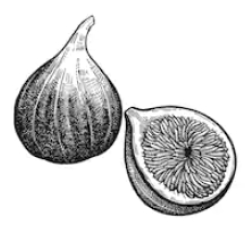
\includegraphics[width=2.5in]{fig1}
\caption{Simulation results for the network.}
\label{fig_1}
\end{figure}







 


 
\begin{table}[!t]
\caption{An Example of a Table\label{tab:table1}}
\centering
\begin{tabular}{|c||c|}
\hline
One & Two\\
\hline
Three & Four\\
\hline
\end{tabular}
\end{table}

 






{\appendix
Please mention whatever prompts and platforms you have used for the project and ideas.}



%{\appendices
%\section*{Proof of the First Zonklar Equation}
%Appendix one text goes here.
% You can choose not to have a title for an appendix if you want by leaving the argument blank
%\section*{Proof of the Second Zonklar Equation}
%Appendix two text goes here.}



 
\end{document}


